
\documentclass{beamer}
\usetheme{Montpellier} 
\usecolortheme{dolphin} 
\usepackage{tikz}
\usepackage{tkz-berge}
\usepackage{parskip}
\setlength{\parskip}{\smallskipamount} 
\usepackage{amsmath}
\usepackage{array}

\title{Extremal Cayley Graphs}
\author{Jordan Blocher, Christopher Linden,  Samantha Hampton}
\date{13 July 2012}
\institute[2008]{REU - Texas State}

 \def\ddd{\displaystyle}
 \def\R{\mbox{$\mathbb R$}}
 \def\Q{\mbox{$\mathbb Q$}}
 \def\Z{\mbox{$\mathbb Z$}}
 \def\N{\mbox{$\mathbb N$}}
 \def\C{\mbox{$\mathbb C$}}


\def\Sym{\operatorname{Sym}}
\def\lcm{\operatorname{lcm}}
\def\adj{\operatorname{adj}}
\def\inc{\operatorname{inc}}
\def\Cay{\operatorname{Cay}}
\def\Geom{\operatorname{\cal G}}
\def\diam{\operatorname{diam}}
\def\rank{\operatorname{rank}}


\begin{document}

\frame{\titlepage}
\frame{
	\frametitle{\underline{Introduction to Cayley Graphs}}
\begin{center}
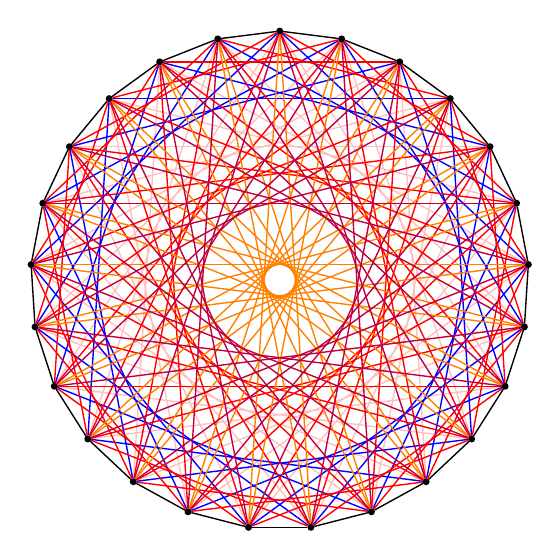
\begin{tikzpicture}[scale=.6]


\GraphInit[vstyle=Simple]
\tikzset{VertexStyle/.append style = {minimum size =2pt, inner sep = 0pt}}


\Vertex[x=187.5pt,y=337.5pt]{0};
\Vertex[x=224.80348307472823pt,y=332.7874741692947pt]{1};
\Vertex[x=259.7630511152573pt,y=318.94600200657953pt]{2};
\Vertex[x=290.1820658893033pt,y=296.8452941132117pt]{3};
\Vertex[x=314.14918882530225pt,y=267.87401924684946pt]{4};
\Vertex[x=330.15847744427305pt,y=233.85254915624213pt]{5};
\Vertex[x=337.2040092642407pt,y=196.91857792939703pt]{6};
\Vertex[x=334.8430876093033pt,y=159.3928028121413pt]{7};
\Vertex[x=323.22405786990294pt,y=123.63310626523908pt]{8};
\Vertex[x=303.0769864163684pt,y=91.88640153769651pt]{9};
\Vertex[x=275.667787843871pt,y=66.14745084375791pt]{10};
\Vertex[x=242.71868290270174pt,y=48.0335271167623pt]{11};
\Vertex[x=206.2999850346457pt,y=38.682794802828326pt]{12};
\Vertex[x=168.70001496535434pt,y=38.682794802828326pt]{13};
\Vertex[x=132.2813170972983pt,y=48.03352711676226pt]{14};
\Vertex[x=99.3322121561291pt,y=66.14745084375782pt]{15};
\Vertex[x=71.92301358363159pt,y=91.88640153769656pt]{16};
\Vertex[x=51.77594213009703pt,y=123.63310626523916pt]{17};
\Vertex[x=40.1569123906967pt,y=159.3928028121413pt]{18};
\Vertex[x=37.795990735759275pt,y=196.91857792939695pt]{19};
\Vertex[x=44.841522555726954pt,y=233.8525491562421pt]{20};
\Vertex[x=60.85081117469775pt,y=267.8740192468495pt]{21};
\Vertex[x=84.81793411069665pt,y=296.8452941132117pt]{22};
\Vertex[x=115.23694888474257pt,y=318.9460020065795pt]{23};
\Vertex[x=150.1965169252717pt,y=332.7874741692946pt]{24};

\SetUpEdge[lw         = .5pt,
            color      = black,
            labelcolor = black]

\Edge(24)(0)
\Edge(0)(1)
\Edge(1)(2)
\Edge(2)(3)
\Edge(3)(4)
\Edge(4)(5)
\Edge(5)(6)
\Edge(6)(7)
\Edge(7)(8)
\Edge(8)(9)
\Edge(9)(10)
\Edge(10)(11)
\Edge(11)(12)
\Edge(12)(13)
\Edge(13)(14)
\Edge(14)(15)
\Edge(15)(16)
\Edge(16)(17)
\Edge(17)(18)
\Edge(18)(19)
\Edge(19)(20)
\Edge(20)(21)
\Edge(21)(22)
\Edge(22)(23)
\Edge(23)(24)

\SetUpEdge[lw         = .5pt,
            color      =pink,
            labelcolor = black]

\Edge(0)(8)
\Edge(2)(10)
\Edge(4)(12)
\Edge(6)(14)
\Edge(8)(16)
\Edge(10)(18)
\Edge(12)(20)
\Edge(14)(22)
\Edge(16)(24)
\Edge(18)(1)
\Edge(20)(3)
\Edge(22)(5)
\Edge(24)(7)
\Edge(1)(9)
\Edge(3)(11)
\Edge(5)(13)
\Edge(7)(15)
\Edge(9)(17)
\Edge(11)(19)
\Edge(13)(21)
\Edge(15)(23)
\Edge(17)(0)
\Edge(19)(2)
\Edge(21)(4)
\Edge(23)(6)

\SetUpEdge[lw         = .5pt,
            color      =blue,
            labelcolor = black]

\Edge(0)(6)
\Edge(6)(12)
\Edge(12)(18)
\Edge(18)(24)
\Edge(24)(5)
\Edge(5)(11)
\Edge(11)(17)
\Edge(17)(23)
\Edge(23)(4)
\Edge(4)(10)
\Edge(10)(16)
\Edge(16)(22)
\Edge(22)(3)
\Edge(3)(9)
\Edge(9)(15)
\Edge(15)(21)
\Edge(21)(2)
\Edge(2)(8)
\Edge(8)(14)
\Edge(14)(20)
\Edge(20)(1)
\Edge(1)(7)
\Edge(7)(13)
\Edge(13)(19)
\Edge(19)(0)

\SetUpEdge[lw         = .5pt,
            color      =red,
            labelcolor = black]

\Edge(0)(4)
\Edge(4)(8)
\Edge(8)(12)
\Edge(12)(16)
\Edge(16)(20)
\Edge(20)(24)
\Edge(24)(3)
\Edge(3)(7)
\Edge(7)(11)
\Edge(11)(15)
\Edge(15)(19)
\Edge(19)(23)
\Edge(23)(2)
\Edge(2)(6)
\Edge(6)(10)
\Edge(10)(14)
\Edge(14)(18)
\Edge(18)(22)
\Edge(22)(1)
\Edge(1)(5)
\Edge(5)(9)
\Edge(9)(13)
\Edge(13)(17)
\Edge(17)(21)
\Edge(21)(0)
\Edge(0)(9)
\Edge(9)(18)
\Edge(18)(2)
\Edge(2)(11)
\Edge(11)(20)
\Edge(20)(4)
\Edge(4)(13)
\Edge(13)(22)
\Edge(22)(6)
\Edge(6)(15)
\Edge(15)(24)
\Edge(24)(8)
\Edge(8)(17)
\Edge(17)(1)
\Edge(1)(10)
\Edge(10)(19)
\Edge(19)(3)
\Edge(3)(12)
\Edge(12)(21)
\Edge(21)(5)
\Edge(5)(14)
\Edge(14)(23)
\Edge(23)(7)
\Edge(7)(16)
\Edge(16)(0)


\SetUpEdge[lw         = .5pt,
            color      = orange,
            labelcolor = black]

\Edge(24)(12)
\Edge(0)(13)
\Edge(1)(14)
\Edge(2)(15)
\Edge(3)(16)
\Edge(4)(17)
\Edge(5)(18)
\Edge(6)(19)
\Edge(7)(20)
\Edge(8)(21)
\Edge(9)(22)
\Edge(10)(23)
\Edge(11)(24)
\Edge(12)(0)
\Edge(13)(1)
\Edge(14)(2)
\Edge(15)(3)
\Edge(16)(4)
\Edge(17)(5)
\Edge(18)(6)
\Edge(19)(7)
\Edge(20)(8)
\Edge(21)(9)
\Edge(22)(10)
\Edge(23)(11)


\SetUpEdge[lw         = .5pt,
            color      = purple,
            labelcolor = black]

\Edge(24)(9)
\Edge(0)(10)
\Edge(1)(11)
\Edge(2)(12)
\Edge(3)(13)
\Edge(4)(14)
\Edge(5)(15)
\Edge(6)(16)
\Edge(7)(17)
\Edge(8)(18)
\Edge(9)(19)
\Edge(10)(20)
\Edge(11)(21)
\Edge(12)(22)
\Edge(13)(23)
\Edge(14)(24)
\Edge(15)(0)
\Edge(16)(1)
\Edge(17)(2)
\Edge(18)(3)
\Edge(19)(4)
\Edge(20)(5)
\Edge(21)(6)
\Edge(22)(7)
\Edge(23)(8)

\end{tikzpicture}
\end{center}

\begin{itemize}
		\item<1->
\begin{center}
Cay($\mathbb{Z}_{25}$, \{$\pm$1,$\pm$4,$\pm$6,$\pm$8, $\pm10$, $\pm$13\})     
\end{center}
                 
\end{itemize}
}

\frame {
	\frametitle{\underline{Introduction to Cayley Graphs}}
	\only<1>{
	\begin{itemize}
                  \item<1-> Definition:  Let $\Gamma$ be a finite group with a subset A. The \underline{\emph{Cayley digraph}}, denoted Cay($\Gamma$,A), is a digraph with vertex set $\Gamma$, such that (x,y) is a directed edge if and only if $yx^{-1}$ $\in$ A

		\item<1->\emph{Cayley digraphs} are vertex transitive.


	\end{itemize}
}
}

\frame {
	\frametitle{\underline{Introduction to Cayley Graphs}}
	\only<1>{
	\begin{itemize}
                  \item<1-> For positive integers $d$ and $k$, we define:
\begin{align*}
m(d,A) &=\max\{m | diam(Cay(\mathbb{Z}_m,A)) \leq d\} \text{,} \\
m(d,k) &= \max_{A: |A| = k}\{m(d,A)  \}.
\end{align*}


	\end{itemize}
}
}


\frame{
	\frametitle{\underline{Introduction to Cayley Graphs}}
	\only<1>{
	\begin{itemize}
                  \item<1-> Current known values include:
\begin{align*}
m(1,k) &= k+1,
\\
\textcolor{blue}{m(2,k)} &\geq \textcolor{blue}{\frac{2}{7}k^2 + O(k)},
\\
m(d,1) &= d+1\text{, and}
\\
m(d,2) &= \left\lfloor \frac{d(d+4)}{3} \right\rfloor+1 \text{ for all } d\geq2.
\end{align*}

	\end{itemize}
}
}

\frame{
\frametitle{\underline{The Pseudocode}}
We begin with 3 generators

\textbf{For each generator }  

\hspace{5mm}create a coefficients table  // $x_1$ $<$ $b_1$ , $x_2$ $<$ c 

\textbf{end}

\textbf{Define} Constant 

\hspace{5mm}Integer $d_{cubed}$ = $diameter * diameter * diameter$
}
\frame{
\frametitle{\underline{The Pseudocode}}
\textbf{Define} Tuples

\hspace{5mm}Tuple $A$ // generators\\
\hspace{5mm}Tuple $Q$  // m coefficients\\
\hspace{5mm}Tuple $x$  // x coefficients

\textbf{Define} Polynomials

\hspace{5mm}Polynomial $X$ // \\
\hspace{5mm}Polynomial $M$  // The bound itself\\
\hspace{5mm}Polynomial $X_{prime}$  // \\ \ \\

\textbf{Define} $M$ a polynomial of $A$ and $Q$
}
\frame{
\frametitle{\underline{The Pseudocode}}
\textbf{Loop} through every choice of $m$ coeffiecient

\hspace{5mm}\textbf{If} $M$ meets criteria // M well formed, less than $d_{cubed}$

\hspace{36mm}// and greater than current best  value

\hspace{10mm}\textbf{Define} $X$ a polynomial of $A$ and $x$

\hspace{10mm}\textbf{Set} Polynomial $X_{prime}$ = $X-M$

\hspace{10mm}\textbf{If} $X$ is well formed

\hspace{15mm}check covering

\hspace{15mm}\textbf{If} covering is $true$

\hspace{20mm}\textbf{Save} the polynomial $M$

\hspace{25mm}$M_{best}  = M$ 

\textbf{end}

}


\frame{
\frametitle{\underline{The Theorem}}
	\only<1>{
	\begin{itemize}
                  \item<1-> 
\begin{theorem}
Let k $\geq$ 17 be an integer. We claim that
 \[
m(2,k) \geq \frac{37}{121}k^2 + O(k). 
\]
\end{theorem}
\end{itemize}
}
}

\frame{
\begin{itemize}
\frametitle{\underline{The Proof}}
\item<1->
Let k $\geq$ 14 be an integer. Let $k_1 = \left \lfloor \frac{k - 6}{11} \right \rfloor$. Let m = $37k_1^2$.  Define 
\begin{align*}
I_0 &= [0, k_1] \ \ \ \ \ \ \ \ \ \ \ \ \ \ \ \ \ \ \ S_0 = \{ik_1 \ |\  i = 0 , 1, ... , k_1 - 1\}\\
I_4 &= [4k_1^2, 4k_1^2+k_1] \ \ \ \ \ \ \ \  S_1 = \{k_1^2 + ik_1 \ |\  i = 0 , 1, ... , k_1 - 1\}\\
I_{15} &= [15k_1^2, 15k_1^2+k_1] \ \ \ \ \ S_2 = \{2k_1^2 + ik_1 \ |\  i = 0 , 1, ... , k_1 - 1\} \\
I_{26} &= [26k_1^2, 26k_1^2+k_1] \ \ \ \ \ S_3 = \{3k_1^2 +ik_1 \ |\   i = 0 , 1, ... , k_1 - 1\}\\ \ \\ 
T_{10} &= \{10k_1^2+ i(k_1 - 1) \ |\   i = 0 , 1, ... , k_1 + 1\}\\
T_{20} &= \{20k_1^2 + i(k_1 - 1) \ |\  i = 0 , 1, ... , k_1 + 1\} \\
T_{30} &= \{30k_1^2 + i(k_1 - 1) \ |\  i = 0 , 1, ... , k_1 + 1\}
\end{align*}

\end{itemize}
}
\frame{
\frametitle{\underline{The Proof}}
Let 
\begin{align*}
T &= T_{10} \cup T_{20} \cup T_{30}\  \ :   \ |T| = 3k_1 + 3 \\
S &= S_{0} \cup S_{1} \cup S_{2} \cup S_{3}  :\ \    |S| = 4k_1\\
I &= I_{0} \cup I_{4} \cup I_{15} \cup I_{26} \ :  \ \ \ |I| = 4k_1 + 4
\end{align*}
Define $A = I \cup S \cup T$, where $|A| \leq 11k_1 + 6 \leq k$. \\
Note that when we write $[\alpha, \beta]$, we mean the integers from $\alpha$ to $\beta$. 

\begin{itemize}
\item<1->
We claim that \textcolor{blue}{A is a 2-basis for $\Z_m$}, such that every element in $\Z_m$ is the sum of two distinct elements in A.
\end{itemize}
}

\frame{
\frametitle{\underline{The Proof}}
\begin{itemize}
\item<1->
We begin by claiming $T_a + I_b$ $\supseteq$ $[(a + b)k_1^2 ,  (a + b + 1)k_1^2]$. \\
\end{itemize}
Let $n \in$ $[(a + b)k_1^2 ,  (a + b + 1)k_1^2]$. Then we can write n as 
\[
n = (a + b) k_1^2 + ck_1 + d \in I_a + T_b 
\]
where $0 \leq c \leq k_1$ and $0 \leq d \leq k_1$.
}


\frame{
\frametitle{\underline{The Proof}}
\underline{Case 1:} \\
If $d \geq c$, then
\[
n = ak_1^2 + c(k_1 + 1) + bk_1^2 + d -  c 
\]
where 
\begin{align*}
ak_1^2 +c(k_1 + 1) &\in T_a \\
 bk_1^2 + (d - c) &\in I_b
\end{align*}
\begin{itemize}
\item<1->
Thus we have $n \in T_a + I_b$. 
\end{itemize}
}


\frame{
\frametitle{\underline{The Proof}}
\underline{Case 2:} \\
If $c>d$, we must have $c \geq 1$, then
\[
n = ak_1^2 + (c - 1)(k_1 + 1) + bk_1^2 + k_1 -c + d + 1, 
\]
where $ak_1^2 + (c - 1)(k_1 + 1) \in T_a$, and $bk_1^2 + k_1 - c + d + 1 \in I_b$.

\vspace{10mm}

\begin{itemize}
\item<1-> Thus we have $n \in T_a + I_b$. 
\end{itemize}
}


\frame{
\frametitle{\underline{The Proof}}
\begin{itemize}
\item<1->
Next we claim that  $S_a + I_b$ $\supseteq$ $[(a + b)k_1^2 ,  (a + b + 1)k_1^2]$. 
\end{itemize}
Let $n \in$ $[(a + b)k_1^2 ,  (a + b + 1)k_1^2]$. Then we can write n as 
\[
n = (a + b) k_1^2 + ck_1 + d = ak_1^2 + ck_1 + bk_1^2 + d
\]
where  $0 \leq c < k_1$ and $0 \leq d \leq k_1$.
\begin{align*}
ak_1^2 + ck_1 &\in S_a \\
bk_1^2 + d &\in I_b
\end{align*} 
\begin{itemize}
\item<1->
Thus we have  $n \in S_a + I_b$
\end{itemize}
}


\frame{
\frametitle{\underline{The Proof}}
\begin{itemize}
\item<1->
Our final claim is $T_a$ + S $\supseteq$ $[(a +1)k_1^2 ,  (a + 4)k_1^2]$. 
\end{itemize}
Let $n \in$ $[(a +1)k_1^2 ,  (a + 4)k_1^2]$. Then we can write n as 
\[
n = (a + b) k_1^2 + ck_1 + d, 
\]
where $1 \leq b \leq 3$, $1 \leq c < k_1$, and $0 \leq d \leq k_1$. 
}


\frame{
\frametitle{\underline{The Proof}}
\underline{Case 1:} \\
If $d > c$, then
\[
n = ak_1^2 + d(k_1 + 1) + (b - 1)k_1^2 + (k_1 + c - d) k_1, 
\]
where 
\begin{align*}
ak_1^2 + d(k_1 + 1) &\in T_a\\
(b - 1)k_1^2 + (k_1 + c - d)k_1 &\in S_{b - 1}
\end{align*}
\begin{itemize}
\item<1->
Thus we have $n \in T_a + S_{b-1}$. 
\end{itemize}
}


\frame{
\frametitle{\underline{The Proof}}
\underline{Case 2: } \\
If $c \geq d$, then
\[
n = ak_1^2 + d(k_1 + 1) + bk_1^2 + (c - d) k_1, 
\]
\begin{align*}
ak_1^2 + d(k_1 + 1) &\in T_a\\
bk_1^2 + (c - d)k_1 &\in S_b
\end{align*}
\begin{itemize}
\item<1->
Thus we have $n \in T_a + S_b$. 
\end{itemize}
}


\frame{
\frametitle{\underline{The Proof}}
Note that
\begin{align*}
8 &\equiv 45\pmod{37},\\
 9 &\equiv 46\pmod{37}, \\
19 &\equiv 56\pmod{37 }.
\end{align*} 
Hence
\begin{align*}
[8k_1^2, 9k_1^2] &= [45k_1^2, 46k_1^2]\\
 [9k_1^2, 10k_1^2] &= [37k_1^2, 38k_1^2]\\
[19k_1^2, 20k_1^2] &= [56k_1^2, 57k_1^2].
\end{align*}
}


\frame{
\frametitle{\underline{The Proof}}
Our interval is covered as follows: 

\begin{align*}
I_0 + S &\supseteq [1, 14k_1^2],\\
I_4 + S &\supseteq [4k_1^2, 8k_1^2],\\
I_{15} + T_{30}  &\supseteq [8k_1^2, 9k_1^2],\\
I_{26} + T_{20}  &\supseteq [9k_1^2, 10k_1^2],\\
T_{10} + I_{0}  &\supseteq [10k_1^2, 11k_1^2],\\
T_{10} + S  &\supseteq [11k_1^2, 14k_1^2],\\
I_{4} + T_{10}  &\supseteq [14k_1^2, 15k_1^2],\\
I_{15} + S  &\supseteq [15k_1^2, 19k_1^2],\\
I_{26} + T_{30}  &\supseteq [19k_1^2, 20k_1^2]
\end{align*}
}


\frame{
\frametitle{\underline{The Proof}}
\begin{align*}
I_{0} + T_{20}  &\supseteq [20k_1^2, 21k_1^2],\\
S + T_{20}  &\supseteq [21k_1^2, 24k_1^2],\\
I_{4} + T_{20}  &\supseteq [24k_1^2, 25k_1^2],\\
I_{15} + T_{10}  &\supseteq [25k_1^2, 26k_1^2],\\
I_{26} + S  &\supseteq [26k_1^2, 30k_1^2],\\
I_{0} + T_{30}  &\supseteq [30k_1^2, 31k_1^2],\\
S + T_{30}  &\supseteq [31k_1^2, 34k_1^2],\\
I_{4} + T_{30}  &\supseteq [34k_1^2, 35k_1^2],\\
I_{15} + T_{20}  &\supseteq [35k_1^2, 36k_1^2], \\
I_{26} + T_{10}  &\supseteq [36k_1^2, 37k_1^2].
\end{align*}
}


\frame{
\frametitle{\underline{The Proof}}
It now follows that 
\[
A + A \supseteq [0, 37k_1^2],
\]
hence
\[
\textcolor{blue}{m(2,k) \geq \frac{37}{121}k^2 + O(k)}. \ \ \ \ \ \qedsymbol
\]


}

\end{document}